\documentclass[handout]{beamer}
\usepackage{pgfpages}
\pgfpagesuselayout{2 on 1}[a4paper,border shrink=5mm]

\usepackage{amsmath,amssymb,amsthm,array}
\usepackage{bm}
\usepackage{multirow}
\usepackage{multicol}
\usepackage{algorithm}
\usepackage{hyperref}
\usepackage{algorithmic}
\usepackage[normalem]{ulem}
\usepackage{fontspec}
\usepackage{numprint}

\setmainfont{CMU Serif}
\setsansfont{CMU Sans Serif}
\newfontfamily{\greekfont}{CMU Serif}
\newfontfamily{\greekfontsf}{CMU Sans Serif}


\usetheme{Rochester}
\usecolortheme{beaver}


\setbeamertemplate{navigation symbols}{}

\title{Το κρυπτοσύστημα RSA} 
\author{Παναγιώτης Γροντάς - Άρης Παγουρτζής}
\date{14/11/2017}
\defbeamertemplate*{footline}{shadow theme}
{%
  \leavevmode%
  \hbox{
		\begin{beamercolorbox}[wd=.4\paperwidth,ht=2.5ex,dp=1.125ex,leftskip=.3cm,rightskip=.3cm plus1fil]{title in head/foot}%
			\usebeamerfont{title in head/foot} RSA  %
		\end{beamercolorbox}
		\begin{beamercolorbox}[wd=.5\paperwidth,ht=2.5ex,dp=1.125ex,leftskip=.3cm,rightskip=.3cm plus1fil]{title in head/foot}%
			\usebeamerfont{title in head/foot} \hfill \insertsection  %
		\end{beamercolorbox}
		\begin{beamercolorbox}[wd=.1\paperwidth,ht=2.5ex,dp=1.125ex,leftskip=.3cm plus1fil,rightskip=.3cm]{author in head/foot}%
			\usebeamerfont{author in head/foot}\insertframenumber\,/\,\inserttotalframenumber
		\end{beamercolorbox}%
  }%
  \vskip0pt%
}
\institute{ΕΜΠ - Κρυπτογραφία (2017-2018)}

 \hypersetup{
  pdfauthor={Panagiotis Grontas},
  pdftitle={RSA},
  colorlinks=true,
  urlcolor=blue,
  linkcolor=white
}
\setlength{\columnseprule}{0.4pt}
\begin{document}
\newcommand{\xor}{ \oplus }
\newcommand{\MSG}{ \mathtt{M} }
\newcommand{\KEY}{ \mathtt{K} }
\newcommand{\CPH}{ \mathtt{C} }
\newcommand{\keygen}{\mathtt{KeyGen}}
\newcommand{\enc}{\mathtt{Encrypt}}
\newcommand{\dec}{\mathtt{Decrypt}}
\newcommand{\adv}{$\mathcal{A} \,$ }
\newcommand{\advb}{$\mathcal{B} \,$ }
\newcommand{\chal}{$\mathcal{C} \,$ }
\newcommand{\cs}{$\mathcal{CS} \,$ }
\newcommand{\zns}{  \mathbb{Z}^*_n }
\newcommand{\zn}{  \mathbb{Z}_n }

\newcommand{\green}[1]{\textcolor{teal}{#1}}
\newcommand{\Green}[1]{\textcolor{Teal}{#1}}
\newcommand{\ForestGreen}[1]{\textcolor{ForestGreen}{#1}}
\newcommand{\blue}[1]{\textcolor{blue}{#1}}
\newcommand{\magenta}[1]{\textcolor{magenta}{#1}}
\newcommand{\cyan}[1]{\textcolor{cyan}{#1}}

\newcommand{\twopartdef}[4]
{ 
		\begin{cases}
			#1 , #2 \\
			#3 , #4
		\end{cases} 
}

\begin{frame}
\titlepage
\end{frame}


\npthousandsep{ }
\begin{frame}{Περιεχόμενα}
\begin{itemize}
\item Κρυπτογραφία Δημοσίου Κλειδιού
\pause
\item Ορισμός RSA
\pause
\item Αριθμοθεωρητικές επιθέσεις
\pause
\item Μοντελοποίηση - Ιδιότητες Ασφάλειας
\pause
\item Παραλλαγές
\end{itemize}
\end{frame}

\section{Ασύμμετρη Κρυπτογραφία}
\begin{frame}[allowframebreaks]{Εισαγωγή}
\begin{block}{Συμμετρικά Κρυπτοσυστήματα - \alert{Το Μειονέκτημα}}
Διανομή Κλειδιών
\end{block}

\begin{block}{Διανομή Κλειδιών σε Συμμετρικά Κρυπτοσυστήματα - Μειονεκτήματα}
\begin{itemize}
\item Πρέπει να 'συναντηθούν' για να ανταλλάξουν κλειδιά 
\item Σε περιβάλλοντα πολλών χρηστών: Ανταλλαγή κλειδιών ανά ζεύγος
\item Για $n$ χρήστες χρειάζονται $\frac{n(n-1)}{2}$ κλειδιά
\item Εύκολο σε ελεγχομένα περιβάλλοντα, δύσκολο σε ανοικτά
\item Δυσκολίες διαχείρισης (πχ. έκδοση νέων), αποθήκευσης
\end{itemize}
\end{block}

\framebreak

\begin{columns}
\column{0.8\textwidth}
\begin{small}
Η λύση μετά από \emph{2500} χρόνια κρυπτογραφίας:  

\medskip

\emph{Whitfield Diffie, Martin Hellman}\\ \href{http://www-ee.stanford.edu/~hellman/publications/24.pdf}{New Directions in Cryptography} - \emph{(1976)}

\medskip
\begin{itemize}
\item Ralph Merkle
\item ίσως και νωρίτερα (GCHQ - James H. Ellis, Clifford Cocks, Malcolm J. Williamson)
\end{itemize}



\begin{block}{Βασική ιδέα}
Ασυμμετρία κρυπτογράφησης - αποκρυπτογράφησης
\end{block}

Παράδειγμα - \magenta{Λουκέτα} 

Κλειδώνουν εύκολα

Aνοίγουν δύσκολα (χωρίς το κλειδί)
 
\end{small}
\column{0.2\textwidth}

\includegraphics[scale=0.3]{padlock.jpg}
\end{columns}

\end{frame}

\begin{frame}{New Directions in Cryptography}

\begin{block}{Ανταλλαγή Κλειδιού Diffie - Hellman}
Δημιουργία κοινού κλειδιού πάνω από δημόσιο - μη ασφαλές κανάλι (online)
\end{block}

\begin{block}{Κρυπτογραφία Δημοσίου Κλειδιού}
Το κλειδί κρυπτογράφησης μπορεί να είναι δημόσιο

Το κλειδί αποκρυπτογράφησης πρέπει να είναι μυστικό

$n$ χρήστες, $n$ ζεύγη κλειδιών

Εύκολη διανομή
\end{block}

\begin{block}{Ψηφιακή Υπογραφή}
Ασύμμετρα MACs

Επαλήθευση με δημόσιο κλειδί - Δημιουργία με ιδιωτικό

Αυθεντικότητα, Μη Αποκήρυξη 
\end{block}

\end{frame}

\begin{frame}{Trapdoor Functions}

\begin{block}{Συναρτήσεις μονής κατεύθυνσης}
Μία συνάρτηση $f$  λέγεται μονής κατεύθυνσης εάν είναι εύκολο να υπολογιστεί το $f(x)$ δεδομένου του $x$, ενώ ο αντίστροφος υπολογισμός του $x$ δεδομένου του $f(x)$ είναι απρόσιτος.
\end{block}
\pause

\begin{block}{Trapdoor Functions - Ορισμός}
Mια συνάρτηση μονής κατεύθυνσης $f$ για την οποία ο υπολογισμός της $f^{−1}$ είναι \emph{εύκολος} όταν δίνεται μια μυστική πληροφορία (secret trapdoor) $k$
\end{block}

\end{frame}

\section{Ορισμός RSA}
\begin{frame}{RSA (1978)}
\begin{itemize}
\item Η πρώτη \emph{κατασκευή} κρυπτοσυστήματος δημοσίου κλειδιού
\item Ron Rivest, Adi Shamir, Leonard Adleman
\item Πατέντα μέχρι το 2000
\end{itemize}

\begin{figure}
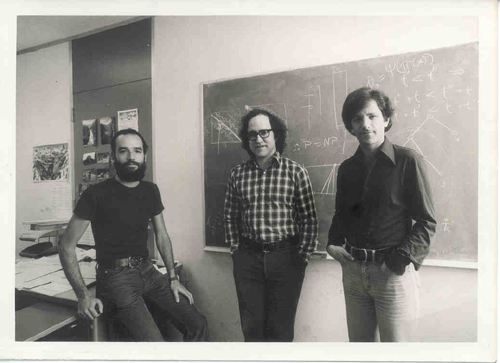
\includegraphics[scale=0.8]{rsa-photo.jpg}  
\end{figure}
\end{frame}

\begin{frame}{Το κρυπτοσύστημα}

 
\textbf{Δημιουργία Κλειδιών:}
\begin{itemize}
\item $KeyGen(1^{\lambda}) = ((e,n),d)$
\item $n=p \cdot q$, 
\\$p,q$ πρώτοι αριθμοί $\frac{\lambda}{2}$ bits
\item Επιλογή $e$ με $1 < e < \phi(n)$ 
και $gcd(e,\phi(n))=1$
\item $d = e^{-1} \pmod{\phi(n)}$ με EGCD
\end{itemize}
\pause
\textbf{Κρυπτογράφηση} 
\begin{itemize}
\item $\enc : \zns \rightarrow \zns$
\item $\enc((e,N), m) = m^e \bmod n$
\end{itemize}
\pause
\textbf{Αποκρυπτογράφηση}
\begin{itemize}
\item $\dec : \zns \rightarrow \zns$
\item $\dec(d, c) = c^d \bmod n$
\end{itemize} 
 
\end{frame}

\begin{frame}{Ορθότητα}
Πρέπει: \green{$\dec(d, \enc((e,n), m)) = m, \forall m$}
\pause
\begin{align*} 
\dec(d, \enc((e,n), m)) = \\  
(m^e)^d \bmod n = \\
 m^{ed} \bmod n = \\
m^{k\phi(n)+1} \bmod n = \\ 
m^{\phi(n)k}  \cdot m  \bmod n = \\ 
m \bmod n
\end{align*}
λόγω Θ.Euler και αφού $m \in \zns$
\end{frame}

\section{Παρατηρήσεις RSA}
\begin{frame}[allowframebreaks]{Κωδικοποίηση Μηνύματος}
Δεν απαιτείται $m \in \zns$ για ορθότητα. Ισχύει για κάθε $m \in \zn$

\framebreak

\begin{block}{Απόδειξη}
$m \in \zn \Rightarrow gcd(m,n) \neq 1 \implies gcd(m,n) \in \{ p,q \}  $

Πρέπει νδο 

$m^{ed} = m \pmod{p}$ και 

$m^{ed} = m \pmod{q}$ 

Από CRT θα έχουμε: 

$m^{ed} = m \bmod{pq}$
\end{block}

\framebreak

\begin{block}{$gcd(m,n)=p$}
\begin{small}
\begin{align*}
m^{ed} = m \pmod{p} \\
(kp)^{ed} = kp = 0 \pmod{p}
\end{align*} \green{OK} 

\begin{align*}
m^{ed} = \green{m} \cdot m^{\green{ed-1}} = m \cdot m^{\green{k\phi(n)}}=  m \cdot m^{k\green{(p-1)(q-1)}} \\
m \cdot m^{\green{{\phi(q)}}k(p-1)} = m \cdot 1 \pmod{q}
\end{align*}
λόγω του Θ. Fermat που ισχύει στο $\mathbb{Z}_q$ \green{OK}
\end{small}
\end{block}
Ομοίως και για $gcd(m,n)=q$

\end{frame}

\begin{frame}{Παράμετρος Ασφάλειας}
\begin{block}{Παραγοντοποίηση Modulus 768bit}
\begin{tiny}

RSA-768 = \alert{\numprint{1230186684530117755130494958384962720772853569595334792197322452151726400507263657518745202199786469389956474942774063845925192557326303453731548268507917026122142913461670429214311602221240479274737794080665351419597459856902143413} }=
\green{\numprint{33478071698956898786044169848212690817704794983713768568912431388982883793878002287614711652531743087737814467999489}}
$\times$
\numprint{36746043666799590428244633799627952632279158164343087642676032283815739666511279233373417143396810270092798736308917}
\end{tiny}
\end{block}
Παραγοντοποιήθηκε το 2009 μετά από 2 ημερολογιακά χρόνια (\href{http://eprint.iacr.org/2010/006}{Factorization of a 768-bit RSA modulus})

2000 χρόνια σε single core system (2.2 GHz AMD Opteron)
\pause 
Χρήση modulus
\begin{itemize}

\item 1024bits: βραχυχρόνια ασφάλεια (80 bit AES key)
\item 2048bits, 3072bits: μακροχρόνια ασφάλεια (~128 bit AES key)
\end{itemize}
\end{frame}

\begin{frame}{Επιλογή πρώτων}
\begin{itemize}
\item Τυχαία επιλογή ακέραιου $\frac{\lambda}{2}$ bits
\pause
\item Primality test (Miller Rabin) επαναληπτικά
\pause
\item $p, q$ ίδιου μήκους
\item $p,q$ safe primes δηλ. $p-1,q-1$ έχουν μεγάλους πρώτους παράγοντες
\item $p+1,q+1$ έχουν μεγάλους πρώτους παράγοντες
\end{itemize}
\end{frame}

\begin{frame}{Επιλογή εκθέτη κρυπτογράφησης}
Θέλουμε \green{ταχύτατη} κρυπτογράφηση
\begin{itemize}
	\item Εύκολος Υπολογισμός Δύναμης Με Square και Multiply
	\pause
	\begin{itemize}
		\item Αναπαράσταση $e$ στο δυαδικό
		\item Για κάθε 0 ύψωση στο τετράγωνο
		\item Για κάθε 1 ύψωση στο τετράγωνο και πολλαπλασιασμός
	\end{itemize}
	\pause
	\item Ελαχιστοποίηση Πολλαπλασιασμών: \green{Low Hamming Weight}	
	\item Παράδειγμα: $e \in \{ \alert{3},\alert{17},65537=2^{16}+1(RFC4871)\}$
	\item Μπορεί $e$ να είναι πρώτος
	\item Ανεξάρτητη επιλογή από $p,q$
\end{itemize}
\end{frame}

\begin{frame}{Βελτίωση αποκρυπτογράφησης}
\alert{Το κλειδί αποκρυπτογράφησης δεν μπορεί να είναι μικρό}
\begin{itemize}
\item Επιθέσεις brute force
\item Εξειδικευμένες επιθέσεις
\item $|d| > \frac{\lambda}{3}$
\end{itemize}
\pause
\begin{block}{Επιτάχυνση}
\begin{itemize}
\item Υπολογισμός $c_p = c \bmod p, c_q = c \bmod q$
\item Υπολογισμός $d_p = d \bmod ({p-1}), \, d_q = d \bmod ({q-1}), $  
\item Υπολογισμός $m_p = c_p^{d_p} \bmod {p}, m_q = c_q^{d_q} \bmod {q} $ 
\item Συνδυασμός με CRT για $m$ 
\end{itemize}
\end{block}
\green{Βελτίωση:4 φορές}
\end{frame}







\section{Ασφάλεια}
\begin{frame}{Σχετιζόμενα (Δύσκολα) Προβλήματα}
\begin{block}{Το πρόβλημα RSA ($e$-οστές ρίζες)}
Δίνονται  $n=pq$, $e$ με $gcd(e,\phi(n))=1$ και $c \in \mathbb{Z}_{n}^*$.

Να βρεθεί η τιμή $c^{\frac{1}{e}(=d)}$
\end{block}
\pause
\begin{block}{To πρόβλημα RSA-KINV}
Δίνονται  $n=pq$, $e$ με $gcd(e,\phi(n))=1$.

Να βρεθεί η τιμή $ e^{-1} \pmod {\phi(n)} (=d)$
\end{block}
\pause
\begin{block}{Το πρόβλημα FACTORING}
Δίνεται $n=pq$ με $p,q$ πρώτοι. Να βρεθούν τα $p,q$
\end{block}
\pause
\begin{block}{Το πρόβλημα COMPUTE-$\phi(n)$}
Δίνεται $n, \phi(n)$ με $n = pq$ όπου $p,q$ πρώτοι.

Να βρεθούν τα $p,q$
\end{block}
\end{frame}

\begin{frame}[allowframebreaks]{Σχέσεις Προβλημάτων}

\begin{block}{RSAP $\leq$ RSA-KINV}
Αν βρεθεί $d=e^{-1}$ υπολογίζεται εύκολα $c^d \bmod n$ 
\end{block}

\begin{block}{RSA-KINV $\leq$ FACTORING}
Έστω ότι μπορούν να βρεθούν $p,q$ για $n=pq$ (λύση FACTORING)

Υπολογισμός $(p-1) \cdot (q-1)$

Χρήση EGCD για εύρεση $\frac{1}{e}$
\end{block}

\framebreak

\begin{block}{COMPUTE-$\phi(n)$ $\equiv$ FACTORING}
$n=pq$ και $\phi(n) = (p-1)(q-1)$

Προκύπτει η εξίσωση 

$p^2 - (n- \phi(n) +1)p + n=0$
\end{block}

\begin{block}{FACTORING $\leq^r$ RSA-KINV (RSA,1977)} 
Αν γνωρίζουμε τον $d=e^{-1}$ μπορούμε να κατασκευάσουμε πιθανοτικό αλγόριθμο παραγοντοποίησης του  $n$ με βάση τον Miller Rabin
\end{block}

\framebreak

Πώς;
\begin{itemize}
\item Υπολογίζουμε $s = ed -1 (=k\phi(n))$
\item $\phi(n),s$ είναι ζυγοί, άρα $s = 2^tr$ με $t \geq 1$ και $r$ μονό
\item Επιλέγουμε τυχαίο $a \in \{1, \cdots n-1 \}$
\item Δύο περιπτώσεις:
\begin{itemize}
    \item $gcd(a,n) > 1$: Βρέθηκε - Τερματισμός
    \item $gcd(a,n) =1$: Από Θ. Euler $a^s =a^ {k\phi(n)} =  1 \pmod n$
\end{itemize}
\item Δηλαδή: $(a^\frac{s}{2})$ \in $\{ 1,-1,+x,-x \}$ $\bmod n$ (τετραγωνικές ρίζες)
\item Αν $(a^\frac{s}{2}) = x \pmod n$ ή τότε $p=gcd(x-1,n)$
\item Αν όχι - επανάληψη με $(a^\frac{s}{4}), \cdots, a^\frac{s}{2^{O(logn)}}$
\item μέχρι να βρεθεί μη τετριμμένη ρίζα
\end{itemize}
 
\end{frame}

\begin{frame}{Σχέσεις Προβλημάτων}
\begin{block}{Συνολική Εικόνα}
RSAP $\leq$ RSA-ΚINV $\leq$ COMPUTE-$\phi(N)$ $\equiv$ FACTORING $\leq^r$ RSA-KINV
\end{block}
\pause
Αργότερα (May, 2004)
FACTORING $\leq$ RSA-KINV
\pause
\begin{block}{Συνολική Εικόνα - Νέα}
RSAP $\leq$ RSA-ΚINV $\equiv$ COMPUTE-$\phi(N) \equiv$ FACTORING
\end{block}
\pause
Το RSAP λοιπόν δεν είναι δυσκολότερο από το FACTORING

Μάλλον είναι ευκολότερο αλλά δεν γνωρίζουμε ακριβώς πόσο.
\pause
\alert{Υπόθεση RSA}: Το RSAP είναι υπολογιστικά απρόσιτο.

\end{frame}

\section{Επιθέσεις}
\begin{frame}{Επίθεση μικρού δημόσιου εκθέτη}
\begin{block}{\alert{Κακή ιδέα}}
Χρήση $e=3$ για να μειωθεί το κόστος κρυπτογράφησης
\end{block}
\pause 
\begin{itemize}
\item Τρία δημόσια κλειδιά $k_1 = (3,n_1), k_2 = (3,n_2), k_3 = (3,n_3)$
\pause
\item O \adv γνωρίζει 3 κρυπτoγραφήσεις του ίδιου μηνύματος $m$
\begin{itemize}
\item $c_1 = \enc(k_1,m) = m^3 \bmod{n_1}$
\item $c_2 = \enc(k_2,m) = m^3 \bmod{n_2}$
\item $c_3 = \enc(k_3,m) = m^3 \bmod{n_3}$
\end{itemize}
\pause
\item Χρήση CRT για υπολογισμό του $c = m^3 \bmod {n_1n_2n_3}$
\item Αλλά $m^3 < n_1n_2n_3$ αφού $m < n_1$ και $m < n_2$ και $ m<n_3$
\item Εύρεση μηνύματος ως $m = \sqrt[3]{c}$
\end{itemize}
\end{frame}

\begin{frame}{Επίθεση μικρού ιδιωτικού εκθέτη - Θεωρία}
\begin{block}{Αναπαράσταση Με Συνεχή Κλάσματα}
Έστω $x \in \mathbb{R}$. Tότε $\exists a_0,a_1,a_2,a_3, \cdots$:
$x = a_0 + \frac{1}{a_1+\frac{1}{a_2+\frac{1}{a_3+\frac{1}{\cdots}}}}$

Αν $x \in \mathbb{Q}$ τότε η αναπαράσταση είναι πεπερασμένη
\end{block}
\pause
\begin{block}{Θεώρημα}
Έστω $x \in \mathbb{R}$. Αν $|x-\frac{a}{b}|<\frac{1}{2b^2}$ τότε το κλάσμα $\frac{a}{b}$ εμφανίζεται στην προσέγγιση με συνεχή κλάσματα του $x$.
\end{block}
\pause
\begin{block}{Βασική ιδέα}
Για μεγάλες τιμές του $e$ (μικρές τιμές του $d$ - \green{$d < \frac{1}{3}n^{\frac{1}{4}}$}) μπορούμε να βρούμε το $d$ μέσω της αναπαράστασης με συνεχή κλάσματα.
\end{block}
\end{frame}

\begin{frame}[allowframebreaks]{Επίθεση μικρού ιδιωτικού εκθέτη - Προσαρμογή} 

\begin{align}
\magenta{n-\phi(n)} = pq - (p-1)(q-1) = p + q -1 < \magenta{3\sqrt{n}}
\end{align}

O \adv γνωρίζει το $e$ και ότι $\exists k: ed  = 1 + k\phi(n)$ 

Επίσης ισχύει 
\begin{align}
e<\phi(n) \Rightarrow  ke < k\phi(n)<1+k\phi(n)=ed \Rightarrow \magenta{k < d}
\end{align}

Επίσης:
\begin{align*}
\magenta{|\frac{e}{n} - \frac{k}{d}|} =   |\frac{ed-kn}{dn}| =  |\frac{1+k\phi(n)-kn}{dn}| = \\ |\frac{1-k(n-\phi(n))}{dn}| \magenta{\leq \frac{1+k(n-\phi(n))}{dn}}
\end{align*}

Από την σχέση (1):
\begin{align*}
|\frac{e}{n} - \frac{k}{d}| < \frac{3k\sqrt{n}}{dn} = \frac{3k}{d\sqrt{n}}
\end{align*}

Από την σχέση (2):
\begin{align*}
|\frac{e}{n} - \frac{k}{d}| <   \frac{3}{\sqrt{n}}
\end{align*}

Από την υπόθεση για το μέγεθος του $d$ έχουμε: 
\begin{align*}
d < \frac{\sqrt[4]{n}}{3} \Rightarrow d^2 < \frac{\sqrt{n}}{9}  \Rightarrow 2d^2 < \frac{2\sqrt{n}}{9} < \frac{\sqrt{n}}{3} \Rightarrow \frac{3}{\sqrt{n}} < \frac{1}{2d^2}
\end{align*}

Τελικά:
\begin{align*}
|\frac{e}{n} - \frac{k}{d}| < \frac{1}{2d^2}
\end{align*}

Επειδή $gcd(k,d)=1$ το κλάσμα $k/d$ είναι απλοποιημένο, και κατά συνέπεια θα εμφανίζεται στην προσέγγιση του $e/n$ με συνεχή κλάσματα.
\end{frame}

\begin{frame}{Επίθεση μικρού ιδιωτικού εκθέτη}
\begin{block}{Διαδικασία}
\begin{itemize}
\item Κρυπτογράφηση μηνύματος $m$ (επιλογής του \adv)
\pause
\item Κατασκευή αναπαράστασης του $e/n$ με συνεχή κλάσματα 
\pause
\item Ύψωση $c$ σε κάθε έναν από τους παρονομαστές της
\pause
\item Επιλογή παρονομαστή που επιτυγχάνει σωστή αποκρυπτογράφηση 
\end{itemize}
\end{block}
\end{frame}

\begin{frame}{Επίθεση μικρού ιδιωτικού εκθέτη - Παράδειγμα}
\begin{small}
$(e,n)=(207031,242537)$

\magenta{Προσεγγίσεις-δοκιμές για $m=8$ και $8^{207031} \bmod 242537 = 46578$}

\begin{columns}
\column{0.5 \textwidth}
\begin{align*}
\frac{207031}{242537} = \textbf{0}+\frac{1}{\frac{242537}{207031}} = \\ 
\textbf{0}+\frac{1}{\textbf{1}+ \frac{35006}{207031}} = \\ 
0+\frac{1}{\textbf{1}+ \frac{1}{\frac{207031}{35006}}} = \\
\textbf{0}+\frac{1}{\textbf{1}+ \frac{1}{\textbf{5}+\frac{32280}{35006}}}  = \\ 
\textbf{0}+\frac{1}{\textbf{1}+ \frac{1}{\textbf{5}+\frac{1}{\textbf{1}+\frac{35006}{32280}}}} = \cdots
\end{align*}
\column{0.5 \textwidth}
\begin{align*}
 \\ 
[0;1] = 0+\frac{1}{1} = 1  \quad \quad \text{και} \\ \quad \quad 46578^1 \bmod 242537 = \alert{46578} \\
[0;1;5] = 0 + \frac{1}{1+\frac{1}{5}} = \frac{5}{6} \quad \quad \text{και}\\ \quad \quad 46578^6 \bmod 242537 = \alert{175938}\\ 
[0;1;5;1] = 0 + \frac{1}{1+\frac{1}{5+1}} = \frac{6}{7} \quad \quad \text{και}\\ \quad \quad 46578^7 \bmod 242537 = \green{8}
\end{align*}
\end{columns}
\end{small}
\end{frame}

\begin{frame}[allowframebreaks]{Επίθεση κοινού γινομένου}
\begin{block}{\alert{Πολύ Κακή ιδέα}}
Χρήση κοινού $n$ για να μειωθεί το κόστος πράξεων modulo
\end{block}
\medskip
\begin{block}{Σενάριο}
TTP διαθέτει $n=pq$ και μοιράζει στους χρήστες $A,B$ τα κλειδιά $(e_A,d_A)$ και $(e_B,d_B)$.
\end{block}
 
Εσωτερική Επίθεση (από γνώστη του $d_A$)
\begin{itemize}
\item Ο $A$ αφού γνωρίζει το $d_A$ μπορεί να παραγοντοποιήσει το $n$ (αναγωγή FACTORING $\leq^r$ RSA-KINV)
\item Υπολογισμός $\phi(N)$
\item Ευρεση  $d_B = e_B^{-1} \pmod{\phi(n)}$ με EGCD
\item Διάβασμα όλων των μηνυμάτων του $B$
\end{itemize}

\framebreak

Εξωτερική Επίθεση
\begin{itemize}
\item Ο \adv  γνωρίζει $(n,e_1),(n,e_2)$
\item Μπορεί να αποκρυπτογραφήσει οποιοδήποτε κοινό μήνυμα $m$
\begin{itemize}
\item $c_1 = m^{e_1} \bmod{n}$
\item $c_2 = m^{e_2} \bmod{n}$
\end{itemize}
\item Αν $gcd(e_1, e_2) = 1$ τότε με τον EGCD μπορούν να βρεθούν αποδοτικά $t_1, t_2$:
\begin{align*}
e_1 t_1 + e_2 t_2 = 1
\end{align*} 
\item $c_1^{t_1}c_2^{t_2} = m^{e_1t_1}m^{e_2t_2}=m^{1}=m$
\end{itemize}
 
\end{frame}

\section{Μοντελοποίηση}
\begin{frame}{To RSA δεν διαθέτει IND-CPA}
\begin{center}
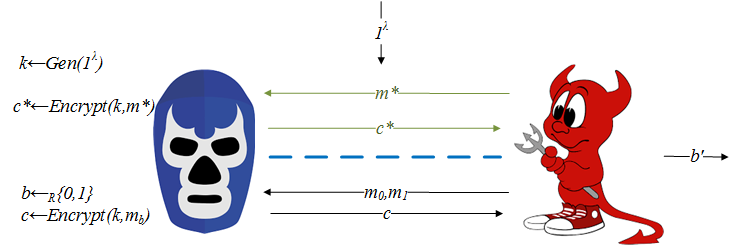
\includegraphics[scale=0.6]{ind-cpa.png}  
\end{center}

\begin{itemize}
\item Γιατί είναι ντετερμινιστικό
\item Ο \adv μπορεί να ξεχωρίσει κρυπτογραφήσεις μηνυμάτων του
\item τις οποίες μπορεί να παράγει μόνος του (δημόσιο κλειδί)
\end{itemize} 
\end{frame}

\begin{frame}[allowframebreaks]{Το RSA δεν διαθέτει IND-CCA(2)}
\begin{center}
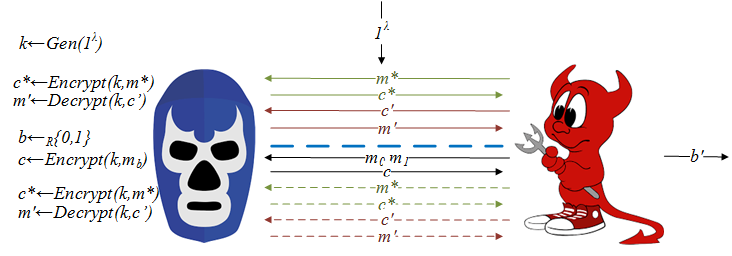
\includegraphics[scale=0.6]{ind-cca.png}  
\end{center}
Αφού δεν διαθέτει IND-CPA (δεν χρειάζεται το decryption oracle)

\framebreak
...αλλά και λόγω \alert{Malleability}
 
\begin{itemize}
\item Στόχος: Αποκρυπτογράφηση του $c = m_b^e \bmod{n}$
\item Μπορεί να αποκρυπτογραφήσει το $ c'= c_b x^e \bmod{n}$ όπου το $x$ είναι δικής του επιλογής
\item Ανακτά το $m_b = \frac{m'}{x}$ 
\item Αν $m_b = m_0$ επιστρέφει $b^*=0$ αλλιώς επιστρέφει $b^*=1$
\end{itemize}
 
\begin{block}{Ομομορφικές ιδιότητες}
$\enc((e,n),m_1) \cdot \enc((e,n),m_2) = m_1^e \cdot m_2^e \bmod{n} = (m_1 \cdot m_2) \bmod{n} = \enc((e,n),m_1 \cdot m_2)$
\end{block}

\end{frame}

\begin{frame}[allowframebreaks]{Διαρροή Πληροφοριών}
\begin{block}{Τι διαρρέει (χωρίς συνέπειες)}
Jacobi symbol
$(\frac{c}{n}) = (\frac{m^e}{n}) = (\frac{m^e}{p}) (\frac{m^e}{q}) =  (\frac{m}{p}) (\frac{m}{q}) = (\frac{m}{n}) $
\end{block}

\begin{block}{Τι δεν διαρρέει}
Έστω $c = m^e \bmod{n}$

$parity((e,n), c) = (m \bmod n) \bmod 2$ - τελευταίο bit του plaintext

$loc((e,n), c) = (m \bmod n) > \frac{n}{2}$ - κάτω μισό / πάνω μισό
\end{block}
\begin{small}

\framebreak

\begin{block}{\green{Θεώρημα (Goldwasser, Micali, Tong)}}
Για κάθε στιγμιότυπο του RSA (e,n), τα παρακάτω είναι ισοδύναμα:
\begin{enumerate}
\item  Υπάρχει ένας αποδοτικός αλγόριθμος \adv τέτοιος ώστε  $\mathcal{A}(c)  = m, \forall m \in \mathbb{Z}_n$ 
\item  Υπάρχει ένας αποδοτικός αλγόριθμος που υπολογίζει την συνάρτηση $parity$
\item  Υπάρχει ένας αποδοτικός αλγόριθμος που υπολογίζει την συνάρτηση $loc$
\end{enumerate}
\end{block}
\end{small}

\framebreak


\green{$parity \rightarrow loc$}
 
\magenta{$loc(c) = parity(c \cdot \enc(2))$} γιατί:

\framebreak

\green{$loc \rightarrow parity$}
 
\magenta{$loc(c) = parity(c \cdot \enc(2))$} γιατί:

$parity( c \cdot \enc(2)) = parity( \enc(2 \cdot m)) = (2m \bmod n) \bmod 2$
\medskip\\

$loc(c)=1 \Rightarrow m > \frac{n}{2} \Rightarrow 2m > n$ δηλ. $(2m \bmod n) \bmod 2 = 1$ αφού $n$ μονός \\και $2m \bmod n = 2m - n$ αφού $n < 2m <2n$\\
\medskip
$loc(c)=0 \Rightarrow m \leq \frac{n}{2}$ τότε $2m \leq n$ δηλ. $(2m \bmod n) \bmod 2 = 0$  

\medskip

\framebreak

\green{$parity \rightarrow loc$}

\magenta{$parity(c) = loc(c \cdot \enc(2^{-1}))$}

Παρατηρώ:

$loc( c \cdot \enc(2^{-1})) = loc(\enc(m \cdot 2^{-1}))  = loc(\enc(m \cdot \frac{n+1}{2}))$ 

\medskip
$parity(c) = 0 \Rightarrow m \bmod 2 =0$  τότε:
$ \frac{m}{2}   < \frac{n}{2} $ αφού $m<n$

\medskip
$parity(c) = 1 \Rightarrow m \bmod 2 =1$  τότε:

$(m \frac{n+1}{2}) \bmod n  = ( (2 k +1) \frac{n+1}{2}) \bmod n  =  k (n+1) + \frac{n+1}{2} \bmod n 
= k + \frac{n+1}{2} > \frac{n}{2}$

\framebreak

\green{Απόδειξη $(1) \Leftrightarrow (2) \Leftrightarrow (3)$}

Προφανώς $(1) \Rightarrow (2)$ (αν μπορώ να αποκρυπτογραφήσω ξέρω parity) και $(2) \Leftrightarrow (3)$ (από προηγούμενα)

Για το $(3) \Rightarrow (1)$

Δυαδική αναζήτηση, για το $m$, χρησιμοποιώντας την $loc$:

\magenta{$loc(\enc(m)) = 0 \iff m \in [0, \frac{n}{2})$} και 

$loc(\enc(2m)) = 0 \iff m \in [0, \frac{n}{4}) \cup (\frac{n}{2}, \frac{3n}{4})$ 

$loc(\enc(4m)) = 0 \iff m \in [0, \frac{n}{8}) \cup (\frac{n}{2}, \frac{5n}{8}) $ 

Άρα αν $loc(\enc(m)) = 0$ και $loc(\enc(2m)) = 0$ και $loc(\enc(4m)) = 0$ τότε $m \in [0, \frac{n}{8})$

$\ldots$ κ.ο.κ.\ για $\log n$ βήματα. 

\end{frame}

\section{Παραλλαγές RSA με IND-CPA}

\begin{frame}[allowframebreaks]{padded-RSA}

\begin{block}{Βασική ιδέα}
\begin{itemize}
    \item Προσθήκη ψηφίων τυχαιοποίησης $r$ στο μήνυμα. 
    \item Κρυπτογράφηση $f(m,r)$
    \item Αποκρυπτογράφηση
    \item Αντιστροφή $f$ (πρέπει να γίνεται εύκολα)
\end{itemize}
\end{block}

\begin{block}{\href{https://tools.ietf.org/html/rfc2313}{PKCS1 v l.5} $f(m,r) = r||m$}
 Έστω $|m|$ = $l$.
\begin{itemize}
\item Πριν την κρυπτογράφηση δημιουργείται το μήνυμα: $\bar{m} = r || m$, όπου $r$ είναι μια τυχαία συμβολοσειρά από $\lambda-l$ bits.
\item Μετατροπή του $\bar{m}$ σε ακέραιο
\item Η κρυπτογράφηση γίνεται (κανονικά) ως: $\bar{c} = \bar{m}^e \bmod n$
\item H αποκρυπτογράφηση γίνεται (κανονικά) ως $\bar{c}^d \bmod n = \bar{m} $
\item Από το $\bar{m}$ κράταμε μόνο τα $l$ bits χαμηλότερης τάξης.
\end{itemize}
\end{block}

Αποδεικνύεται ότι διαθέτει ασφάλεια IND-CPA, όχι όμως IND-CCA (μπορούμε να εκμεταλλευτούμε την δομή του μηνύματος)
\end{frame}

\begin{frame}[allowframebreaks]{Η επίθεση του Bleichenbacher (Million Message Attack)}

\begin{block}{\green{Βασική Ιδέα}:Padding Oracle}
Χρήση ενός συστήματος το οποίο μπορεί να αποφανθεί αν ένα κρυπτοκείμενο έχει προκύψει με σωστό padding
\end{block}

\begin{itemize}
\item Ακριβής Μορφή padded μηνύματος στο PKCS1: $PKCS(r,m)= \mathsf{0x} \;\; \mathtt{ 00 || 02 || r || 00 || m}$
\item Αποκρυπτογράφηση: 
\begin{itemize}
\item Έλεγχος πρώτου byte για την τιμή $0$
\item Έλεγχος δεύτερου byte για την τιμή $2$
\item Αναζήτηση του $0$ 
\item Ανάκτηση του $m$
\end{itemize}
\framebreak
\item To oracle στην πράξη:
\begin{itemize} 
\item Ύπαρξη μηνύματος λάθους για μη αποδεκτό padding ή 
\item ανάκτηση της πληροφορίας μέσω side channel (πχ. χρόνος απάντησης)
\end{itemize}
\end{itemize}

\begin{block}{Fact}
Μια τυχαία συμβολοσειρά από bytes θα έχει την σωστή μορφή δηλ. 
$$\mathsf{0x} \;\; \mathtt{ 00 || 02 || \text{non-zero} || 00 || \text{non-zero}}$$
με πιθανότητα από $2^{-17}$ εώς $2^{-15}$.
\end{block}

\framebreak 
Η επίθεση:
\begin{itemize}
\item Στόχος: Αποκρυπτογράφηση ενός $c$ 
\item Ο \adv ξέρει ότι $c= PKCS(r,m)^e \bmod{n}$
\item Διαλέγει \emph{πολλά} τυχαία $s$
\item Στέλνει στο padding oracle μηνύματα της μορφής $ c'= c s^e \bmod{n}$ 
\item Λόγω ιδιοτήτων RSA: $c' = (s PKCS(r,m))^e \bmod{n}$
\item Στα περισσότερα η αποκρυπτογράφηση δίνει λάθος padding
\framebreak
\item Αν \emph{δεν} δώσει:
\begin{itemize} 
\item Ξέρουμε ότι το padded plaintext έχει σωστή μορφή
\item Δηλαδή το $sPKCS(r,m)$ βρίσκεται σε ένα συγκεκριμένο εύρος τιμών (ξεκινούν με 0002)
\item Τροποποίηση του $s$ ώστε να περιορίζεται το εύρος της αναζήτησης
\item Επανάληψη
\end{itemize} 
\item Με 300.000 εως 2.000.000 $c'$ μπορεί να αποκρυπτογραφηθεί το $c$ 
\end{itemize}

\begin{block}{Λύσεις}
\begin{itemize}
    \item Αφαίρεση μηνύματος λάθους για padding
    \item Τροποποίηση ώστε να υπάρχει ασφάλεια IND-CCA2 
\end{itemize}

\magenta{Ιδέες;}

\end{block}


\end{frame}

\begin{frame}[allowframebreaks]{RSA-OAEP (PKCS1 v2.0)}
\begin{block}{Βασική Ιδέα}
Τα τυχαία bits πρέπει να 'διαχυθούν' σε όλο το κρυπτοκείμενο \\
(\magenta{Δίκτυα Feistel}) \\
Πρέπει να υπάρχει κάποιου είδους δέσμευση στο αρχικό μήνυμα ενσωματωμένη στο κρυπτοκείμενο \\
(\magenta{Συνάρτηση Σύνοψης})
\end{block}

\begin{block}{Υποθέσεις}
\begin{itemize}
\item $|m|$ = $l$
\item $\mathcal{G}, \mathcal{H} : \{0,1\}^{2l} \rightarrow \{0,1\}^{2l}$ συναρτήσεις σύνοψης
\item $r \in \{0,1\}^{2l}$
\end{itemize}
\end{block}


\framebreak 
 
\begin{block}{Κρυπτογράφηση}
\begin{itemize}
\item Padding για μέγεθος $2l$: $m' = m || 0^l$
\item Διάχυση bits τυχαιότητας $m_1 = \mathcal{G}(r) \xor m'$
\item Δέσμευση $m_2 = r \xor \mathcal{H}(m_1)$
\item Συνδυασμός $\bar{m} = m_1 || m_2$
\item Κρυπτογράφηση $\bar{c} = \bar{m}^e \bmod n$
\end{itemize}
\end{block}

\framebreak 

\begin{block}{Αποκρυπτογράφηση}
\begin{itemize}
\item Αποκρυπτογράφηση $\bar{c}^d \bmod n = \bar m$
\item Θεωρούμε ότι $\bar{m} = m_1 || m_2$ (χωρισμός στα δύο)
\item $\mathcal{H}(m_1) \xor m_2$
\item Ανακτούμε το $r$ (\magenta{γιατί;})
\item $m_1 \xor \mathcal{G}(r)$
\item Ανακτούμε το $m'$
\item Έλεγχος $l$ bits χαμηλότερης τάξης
\item Αν είναι 0 τότε ανάκτηση μηνύματος από τα $l$ bits υψηλότερης τάξης
\end{itemize}
\end{block}

\framebreak 

\begin{figure}
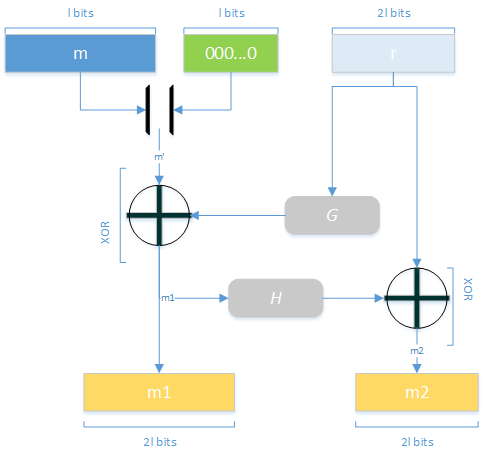
\includegraphics[scale=0.6]{oaep.png}  
\end{figure}

\end{frame}

\section{Πηγές}
\begin{frame}{Βιβλιογραφία}
\begin{tiny}
\begin{enumerate}
\item St. Zachos and Aris Pagourtzis. Στοιχεία Θεωρίας Αριθμών και Εφαρμογές στην Κρυπτογραφία. Πανεπιστημιακές Σημειώσεις
\item Jonathan Katz and Yehuda Lindell. Introduction to Modern Cryptography (Chapman and Hall/Crc Cryptography and Network Security Series). Chapman
and Hall/CRC, 2007
\item \href{http://goo.gl/b75I29}{Nigel Smart. Introduction to cryptography} 
\item Paar, Christof, and Jan Pelzl. Understanding cryptography: a textbook for students and practitioners. Springer Science-Business Media, 2009.
\item Dan Boneh, Introduction to cryptography, online course
\medskip
\item R.L. Rivest, A. Shamir, and L. Adleman. \href{https://people.csail.mit.edu/rivest/Rsapaper.pdf}{A method for obtaining digital signatures and public-key cryptosystems}. Communications of the ACM,
21:120–126, 1978
\item  Alexander May. \href{https://www.iacr.org/archive/crypto2004/31520213/det.pdf}{Computing the rsa secret key is deterministic polynomial time equivalent to factoring}. In Advances in Cryptology–CRYPTO 2004,
pages 213–219. Springer, 2004.
\item Michael J Wiener. \href{http://igm.univ-mlv.fr/~jyt/Crypto/4/10.1.1.92.5261.pdf}{Cryptanalysis of short rsa secret exponents}. Information Theory, IEEE Transactions on, 36(3):553–558, 1990.
\item Boneh, Dan. \href{http://www.ams.org/notices/199902/boneh.pdf}{"Twenty years of attacks on the RSA cryptosystem."} Notices of the AMS 46.2 (1999): 203-213.
\item Bellare, Mihir, and Phillip Rogaway. \href{https://cseweb.ucsd.edu/~mihir/papers/oae.pdf}{"Optimal asymmetric encryption."} Advances in Cryptology—EUROCRYPT'94. Springer Berlin Heidelberg, 1995.
\item Bleichenbacher, Daniel. \href{http://archiv.infsec.ethz.ch/education/fs08/secsem/Bleichenbacher98.pdf}{"Chosen ciphertext attacks against protocols based on the RSA encryption standard PKCS1"} Advances in Cryptology—CRYPTO'98. Springer Berlin Heidelberg, 1998.
\end{enumerate}
\end{tiny}
\end{frame}

 
\end{document}
\end{frame}